\section{Lecture 2: Rotation, Lie Groups, SE(3), SE\texorpdfstring{$_2$}{2}(3), and Quaternions}
\label{sec:lecture02}

\paragraph{Further reading.} This lecture draws on several standard references: matrix Lie groups in Barfoot~\cite[Ch.~7]{Barfoot2017StateEstimation}; the Lie-group treatment of $SO(3)$/$SE(3)$ in the GTSAM notes~\cite{DellaertGTSAMLieGroups}, Atanasov's ECE276A slides~\cite{Atanasov2020SO3SE3}, and the micro Lie theory of Sol\`a, Deray \& Atchuthan~\cite{Sola2018MicroLie}; and quaternion algebra/kinematics in Trawny \& Roumeliotis~\cite[Sec.~1]{Trawny2005Quaternion} and Sol\`a~\cite[Sec.~1--3]{Sola2017Quaternion}.

% =====================================================================
\subsection{Preliminaries: useful series}
The matrix exponential and the sine/cosine series underpin everything that follows:
\begin{align}
e^{x} = \exp(x) &= \sum_{k=0}^{\infty}\frac{1}{k!}x^{k} \\
&= I + x + \tfrac{1}{2!}x^{2} + \tfrac{1}{3!}x^{3} + \tfrac{1}{4!}x^{4} + \cdots, \\
\sin(x) &= \sum_{k=0}^{\infty}\frac{(-1)^{k}}{(2k+1)!}x^{2k+1} \\
&= x - \tfrac{1}{3!}x^{3} + \tfrac{1}{5!}x^{5} - \cdots, \\
\cos(x) &= \sum_{k=0}^{\infty}\frac{(-1)^{k}}{(2k)!}x^{2k} \\
&= 1 - \tfrac{1}{2!}x^{2} + \tfrac{1}{4!}x^{4} - \cdots.
\end{align}
For small $x$ (so that $x^2,x^3\to 0$), the important first-order approximations are $e^{x}\approx I + x$, $\sin(x)\approx x$, and $\cos(x)\approx 1$.

% =====================================================================
\subsection{Frames, notation, and transformations}

We work with coordinate frames $\{A\}$ and $\{B\}$. A point/vector $\vect{L}$ expressed in $\{A\}$ is ${}^{A}\vect{L}$, and in $\{B\}$ is ${}^{B}\vect{L}$. The angle $\theta_{A\to B}$ is the rotation about the $z$-axis taking $\{A\}$ to $\{B\}$ (Fig.~\ref{fig:lec02-frames}).

\begin{figure}[H]
\centering
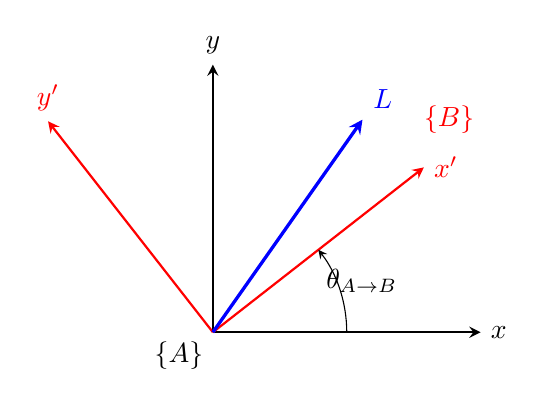
\begin{tikzpicture}[>=stealth,scale=1.0]
  % Frame {A}
  \draw[->,thick] (0,0) -- (3.4,0) node[right] {$x$};
  \draw[->,thick] (0,0) -- (0,3.4) node[above] {$y$};
  \node[below left] at (0,0) {$\{A\}$};
  % Frame {B}, rotated by theta
  \draw[->,thick,red,rotate=38] (0,0) -- (3.4,0) node[right] {$x'$};
  \draw[->,thick,red,rotate=38] (0,0) -- (0,3.4) node[above] {$y'$};
  \node[red] at (3.0,2.7) {$\{B\}$};
  % angle arc
  \draw[->] (1.7,0) arc (0:38:1.7);
  \node at (19:2.0) {$\theta_{A\to B}$};
  % vector L
  \draw[->,very thick,blue] (0,0) -- (1.9,2.7) node[above right] {$\vect{L}$};
\end{tikzpicture}
\caption{Frame $\{B\}$ is frame $\{A\}$ rotated by $\theta_{A\to B}$ about the $z$-axis; the vector $\vect{L}$ can be expressed in either frame.}
\label{fig:lec02-frames}
\end{figure}

The rotation matrix ${}^{A}_{B}\vect{R}$ maps a vector from $\{B\}$ to $\{A\}$:
\begin{align}
{}^{A}\vect{L} &= {}^{A}_{B}\vect{R}\,{}^{B}\vect{L} \\
&= {}^{A}_{B}\vect{R}(\theta_{A\to B})\,{}^{B}\vect{L}.
\end{align}
Adding the translation ${}^{A}\vect{p}_{B}$ (the origin of $\{B\}$ expressed in $\{A\}$, Fig.~\ref{fig:lec02-transl}) gives the full rigid-body transformation
\begin{align}
\{A\},\{B\} \;\Rightarrow\; \big\{\,{}^{A}_{B}\vect{R},\;{}^{A}\vect{p}_{B}\big\} \;\Rightarrow\;
{}^{A}_{B}\vect{T} = \begin{bmatrix} {}^{A}_{B}\vect{R} & {}^{A}\vect{p}_{B} \\ \vect{0}_{1\times3} & 1 \end{bmatrix}.
\end{align}

\begin{figure}[H]
\centering
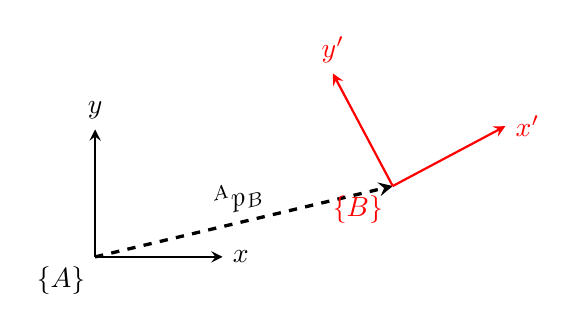
\begin{tikzpicture}[>=stealth,scale=0.9]
  % Frame A
  \draw[->,thick] (0,0) -- (1.8,0) node[right] {$x$};
  \draw[->,thick] (0,0) -- (0,1.8) node[above] {$y$};
  \node[below left] at (0,0) {$\{A\}$};
  % translation vector
  \draw[->,very thick,dashed] (0,0) -- (4.2,1.0) node[midway,above,sloped] {${}^{A}\vect{p}_{B}$};
  % Frame B
  \begin{scope}[shift={(4.2,1.0)},rotate=28]
    \draw[->,thick,red] (0,0) -- (1.8,0) node[right] {$x'$};
    \draw[->,thick,red] (0,0) -- (0,1.8) node[above] {$y'$};
    \node[red,below left] at (0,0) {$\{B\}$};
  \end{scope}
\end{tikzpicture}
\caption{A rigid-body transformation combines the rotation ${}^{A}_{B}\vect{R}$ with the translation ${}^{A}\vect{p}_{B}$.}
\label{fig:lec02-transl}
\end{figure}

% =====================================================================
\subsection{Defining rotation}

\paragraph{Euler angles.}
With roll $\theta$ (about $x$), pitch $r$ (about $y$), yaw $\psi$ (about $z$),
\begin{align}
\vect{R}(\theta) = \begin{bmatrix} 1 & 0 & 0 \\ 0 & \cos\theta & -\sin\theta \\ 0 & \sin\theta & \cos\theta \end{bmatrix},\;
\vect{R}(r) = \begin{bmatrix} \cos r & 0 & \sin r \\ 0 & 1 & 0 \\ -\sin r & 0 & \cos r \end{bmatrix},\;
\vect{R}(\psi) = \begin{bmatrix} \cos\psi & -\sin\psi & 0 \\ \sin\psi & \cos\psi & 0 \\ 0 & 0 & 1 \end{bmatrix},
\end{align}
and the yaw--pitch--roll composition is
\begin{align}
\vect{R} &= \vect{R}(\psi)\,\vect{R}(r)\,\vect{R}(\theta) \\
&= \begin{bmatrix} \cos\psi & -\sin\psi & 0 \\ \sin\psi & \cos\psi & 0 \\ 0 & 0 & 1 \end{bmatrix}
\begin{bmatrix} \cos r & 0 & \sin r \\ 0 & 1 & 0 \\ -\sin r & 0 & \cos r \end{bmatrix}
\begin{bmatrix} 1 & 0 & 0 \\ 0 & \cos\theta & -\sin\theta \\ 0 & \sin\theta & \cos\theta \end{bmatrix}.
\end{align}

\paragraph{Infinitesimal rotation and the skew-symmetric matrix.}
For small angles $\delta\theta,\delta r,\delta\psi\to 0$ each elementary rotation linearizes ($\cos\to1$, $\sin\to$ angle):
\begin{align}
\vect{R}(\delta\theta) = \begin{bmatrix} 1 & 0 & 0 \\ 0 & 1 & -\delta\theta \\ 0 & \delta\theta & 1 \end{bmatrix},\quad
\vect{R}(\delta r) = \begin{bmatrix} 1 & 0 & \delta r \\ 0 & 1 & 0 \\ -\delta r & 0 & 1 \end{bmatrix},\quad
\vect{R}(\delta\psi) = \begin{bmatrix} 1 & -\delta\psi & 0 \\ \delta\psi & 1 & 0 \\ 0 & 0 & 1 \end{bmatrix}.
\end{align}
Multiplying the last two and dropping all second-order products ($\delta r\,\delta\theta\approx0$ etc.),
\begin{align}
\vect{R}(\delta r)\vect{R}(\delta\theta)
&= \begin{bmatrix} 1 & 0 & \delta r \\ 0 & 1 & 0 \\ -\delta r & 0 & 1 \end{bmatrix}
\begin{bmatrix} 1 & 0 & 0 \\ 0 & 1 & -\delta\theta \\ 0 & \delta\theta & 1 \end{bmatrix} \\
&= \begin{bmatrix} 1 & 0 & \delta r \\ 0 & 1 & -\delta\theta \\ -\delta r & \delta\theta & 1 \end{bmatrix},
\end{align}
and then
\begin{align}
\vect{R} = \vect{R}(\delta\psi)\vect{R}(\delta r)\vect{R}(\delta\theta)
&= \begin{bmatrix} 1 & -\delta\psi & 0 \\ \delta\psi & 1 & 0 \\ 0 & 0 & 1 \end{bmatrix}
\begin{bmatrix} 1 & 0 & \delta r \\ 0 & 1 & -\delta\theta \\ -\delta r & \delta\theta & 1 \end{bmatrix} \notag\\
&= \begin{bmatrix} 1 & -\delta\psi & \delta r \\ \delta\psi & 1 & -\delta\theta \\ -\delta r & \delta\theta & 1 \end{bmatrix} \\
&= \vect{I} + \begin{bmatrix} 0 & -\delta\psi & \delta r \\ \delta\psi & 0 & -\delta\theta \\ -\delta r & \delta\theta & 0 \end{bmatrix} \\
&= \vect{I} + \skewsym{\vect{\theta}},
\end{align}
where the small-angle vector is $\vect{\theta} = [\delta\theta,\;\delta r,\;\delta\psi]\trans$. The matrix $\skewsym{\vect{\theta}}$ is skew-symmetric, $\skewsym{\vect{\theta}} = -\skewsym{\vect{\theta}}\trans$. This motivates writing a finite rotation as $\vect{R}(\vect{\theta}) \approx \vect{I} + \skewsym{\vect{\theta}} \approx \exp(\skewsym{\vect{\theta}})$, and defining $\Exp(\vect{\theta}) \triangleq \exp(\skewsym{\vect{\theta}})$. The question is then whether $\vect{R}(\vect{\theta}) = \Exp(\vect{\theta})$.

% =====================================================================
\subsection{Axis--angle and Rodrigues' formula}

Let $\vect{k}$ be the unit rotation axis and $\theta$ the rotation angle, with $\vect{\theta} = \theta\vect{k} = [\theta_1,\theta_2,\theta_3]\trans$, so
\begin{align}
\vect{k} = \begin{bmatrix} k_1 \\ k_2 \\ k_3 \end{bmatrix},\quad
\skewsym{\vect{k}} = \begin{bmatrix} 0 & -k_3 & k_2 \\ k_3 & 0 & -k_1 \\ -k_2 & k_1 & 0 \end{bmatrix},\quad
\skewsym{\vect{\theta}} = \begin{bmatrix} 0 & -\theta_3 & \theta_2 \\ \theta_3 & 0 & -\theta_1 \\ -\theta_2 & \theta_1 & 0 \end{bmatrix}.
\end{align}
The skew operator on a unit vector satisfies the cyclic power identities
\begin{align}
\skewsym{\vect{k}}^{2} &= \vect{k}\vect{k}\trans - \vect{I}_3, &
\skewsym{\vect{k}}^{3} &= -\skewsym{\vect{k}}, &
\skewsym{\vect{k}}^{4} &= -\skewsym{\vect{k}}^{2}, \\
\skewsym{\vect{k}}^{5} &= \skewsym{\vect{k}}, &
\skewsym{\vect{k}}^{6} &= \skewsym{\vect{k}}^{2}, &
\skewsym{\vect{k}}^{7} &= -\skewsym{\vect{k}}.
\end{align}
Substituting $\skewsym{\vect{\theta}} = \theta\skewsym{\vect{k}}$ into the exponential series term by term,
\begin{align}
\Exp(\vect{\theta}) = \exp(\theta\skewsym{\vect{k}})
&= \vect{I} + \theta\skewsym{\vect{k}} + \tfrac{\theta^2}{2!}\skewsym{\vect{k}}^2 + \tfrac{\theta^3}{3!}\skewsym{\vect{k}}^3 + \tfrac{\theta^4}{4!}\skewsym{\vect{k}}^4 \notag\\
&\quad + \tfrac{\theta^5}{5!}\skewsym{\vect{k}}^5 + \tfrac{\theta^6}{6!}\skewsym{\vect{k}}^6 + \tfrac{\theta^7}{7!}\skewsym{\vect{k}}^7 + \cdots \notag\\
&= \vect{I} + \theta\skewsym{\vect{k}} + \tfrac{\theta^2}{2!}\skewsym{\vect{k}}^2 - \tfrac{\theta^3}{3!}\skewsym{\vect{k}} - \tfrac{\theta^4}{4!}\skewsym{\vect{k}}^2 \notag\\
&\quad + \tfrac{\theta^5}{5!}\skewsym{\vect{k}} + \tfrac{\theta^6}{6!}\skewsym{\vect{k}}^2 - \tfrac{\theta^7}{7!}\skewsym{\vect{k}} + \cdots \notag\\
&= \vect{I} + \underbrace{\big(\theta - \tfrac{\theta^3}{3!} + \tfrac{\theta^5}{5!} - \tfrac{\theta^7}{7!} + \cdots\big)}_{\sin\theta}\skewsym{\vect{k}} \notag\\
&\quad + \underbrace{\big(\tfrac{\theta^2}{2!} - \tfrac{\theta^4}{4!} + \tfrac{\theta^6}{6!} - \cdots\big)}_{1-\cos\theta}\skewsym{\vect{k}}^2,
\end{align}
which gives \textbf{Rodrigues' rotation formula}
\begin{empheq}[box=\fbox]{align}
\vect{R}(\vect{\theta}) = \Exp(\vect{\theta}) = \exp(\theta\skewsym{\vect{k}})
= \vect{I} + \sin\theta\,\skewsym{\vect{k}} + (1-\cos\theta)\,\skewsym{\vect{k}}^2.
\end{empheq}
For a small angle $\delta\theta\to0$, $\vect{R}(\delta\vect{\theta}) \approx \vect{I} + \skewsym{\delta\vect{\theta}}$ (small-angle approximation).

\paragraph{Logarithmic map.}
The log map is the inverse of the exponential map:
\begin{align}
\log(\vect{R}) = \skewsym{\vect{\theta}}, \quad \Log(\vect{R}) = \vect{\theta}_{3\times1}, \qquad
\theta = \arccos\!\Big(\tfrac{\tr\vect{R} - 1}{2}\Big), \quad \skewsym{\vect{k}} = \frac{\vect{R} - \vect{R}\trans}{2\sin\theta}.
\end{align}

% =====================================================================
\subsection{SO(3) kinematics}

The two directions of the maps are: from the vector space $\Reals^3$ via the Lie algebra to the Lie group, $\vect{\theta} \to \skewsym{\vect{\theta}} \to \vect{R} = \Exp(\vect{\theta})$; and back, $\vect{R} \to \skewsym{\vect{\theta}} \to \vect{\theta} = \Log(\vect{R})$.

\paragraph{(1) Angular-velocity kinematics.} Differentiating the orthogonality constraint $\vect{R}\vect{R}\trans = \vect{I}_3$,
\begin{align}
\frac{\mathrm{d}}{\mathrm{d}t}(\vect{R}\vect{R}\trans) = \vect{0}
\;\Rightarrow\; \dot{\vect{R}}\vect{R}\trans + \vect{R}\dot{\vect{R}}\trans = \vect{0}
\;\Rightarrow\; \dot{\vect{R}}\vect{R}\trans = -\vect{R}\dot{\vect{R}}\trans = -(\dot{\vect{R}}\vect{R}\trans)\trans,
\end{align}
so $\dot{\vect{R}}\vect{R}\trans$ is skew-symmetric. Writing it as $\skewsym{\vect{\omega}}$ with $\skewsym{\vect{\omega}} = \begin{bmatrix} 0 & -\omega_3 & \omega_2 \\ \omega_3 & 0 & -\omega_1 \\ -\omega_2 & \omega_1 & 0 \end{bmatrix}$,
\begin{align}
\dot{\vect{R}}\vect{R}\trans = \skewsym{\vect{\omega}} \;\Rightarrow\; \dot{\vect{R}} = \skewsym{\vect{\omega}}\vect{R}.
\end{align}

\paragraph{(2) Equivalent limit form.} With $\vect{R}(t+\Delta t) = \vect{R}(t)\exp(\skewsym{\vect{\omega}}\Delta t)$,
\begin{align}
\dot{\vect{R}}(t) &= \lim_{\Delta t\to0}\frac{\vect{R}(t+\Delta t) - \vect{R}(t)}{\Delta t} \\
&= \lim_{\Delta t\to0}\frac{\vect{R}(t)\exp(\skewsym{\vect{\omega}}\Delta t) - \vect{R}(t)}{\Delta t} \\
&= \vect{R}(t)\lim_{\Delta t\to0}\frac{\exp(\skewsym{\vect{\omega}}\Delta t) - \vect{I}}{\Delta t} \\
&= \vect{R}(t)\skewsym{\vect{\omega}}.
\end{align}

\paragraph{(3) Integration.} With $\vect{R}_i = \exp(\skewsym{\vect{\omega}_i}\Delta t_i)$, composing increments gives
\begin{align}
\vect{R}_{1\to k} &= \vect{R}_k\vect{R}_{k-1}\cdots\vect{R}_2\vect{R}_1 \\
&= \exp(\skewsym{\vect{\omega}_k}\Delta t_k)\cdots\exp(\skewsym{\vect{\omega}_1}\Delta t_1).
\end{align}

\paragraph{(4) Interpolation.} For ${}^{G}_{t_1}\vect{R},{}^{G}_{t_2}\vect{R}$ and $t\in[t_1,t_2]$, define the relative rotation and its angle, and the interpolation ratio:
\begin{align}
{}^{t_1}_{t_2}\vect{R} &= {}^{G}_{t_1}\vect{R}\trans\,{}^{G}_{t_2}\vect{R}, \\
{}^{t_1}_{t_2}\vect{\theta} &= \Log({}^{t_1}_{t_2}\vect{R}) = \Log({}^{G}_{t_1}\vect{R}\trans\,{}^{G}_{t_2}\vect{R}), \\
\lambda &= \frac{t-t_1}{t_2-t_1}.
\end{align}
Then
\begin{align}
{}^{G}_{t}\vect{R} &= {}^{G}_{t_1}\vect{R}\,{}^{t_1}_{t}\vect{R} \\
&= {}^{G}_{t_1}\vect{R}\,\Exp\!\big(\lambda\,{}^{t_1}_{t_2}\vect{\theta}\big).
\end{align}

\paragraph{(5) Right Jacobian.} For a rotation $\vect{R}(\vect{\theta}) = \Exp(\vect{\theta})$, perturb the angle by $\delta\vect{\theta}\in\Reals^3$ and let $\delta\vect{\varphi}$ be the corresponding small rotation in $\mathfrak{so}(3)$:
\begin{align}
\vect{R}(\vect{\theta})\,\Exp(\delta\vect{\varphi}) = \vect{R}(\vect{\theta}+\delta\vect{\theta})
\;\Rightarrow\;
\Exp(\vect{\theta})\Exp(\delta\vect{\varphi}) = \Exp(\vect{\theta}+\delta\vect{\theta}).
\end{align}
Solving for $\delta\vect{\varphi}$,
\begin{align}
\Exp(\delta\vect{\varphi}) = \Exp(\vect{\theta})^{-1}\Exp(\vect{\theta}+\delta\vect{\theta})
\;\Rightarrow\;
\delta\vect{\varphi} = \Log\!\big(\Exp(\vect{\theta})^{-1}\Exp(\vect{\theta}+\delta\vect{\theta})\big),
\end{align}
and the \emph{right Jacobian} is the derivative of $\delta\vect{\varphi}$ with respect to $\delta\vect{\theta}$:
\begin{align}
\vect{J}_r(\vect{\theta}) \triangleq \frac{\partial\,\delta\vect{\varphi}}{\partial\,\delta\vect{\theta}}
= \lim_{\delta\vect{\theta}\to0}\frac{\Log\!\big(\Exp(\vect{\theta})^{-1}\Exp(\vect{\theta}+\delta\vect{\theta})\big)}{\delta\vect{\theta}}.
\end{align}
Equivalently, $\Exp(\vect{\theta}+\delta\vect{\theta}) = \Exp(\vect{\theta})\Exp\!\big(\vect{J}_r(\vect{\theta})\,\delta\vect{\theta}\big)$, and inverting,
\begin{align}
\Exp(\vect{\theta})\Exp(\delta\vect{\varphi}) = \Exp\!\big(\vect{\theta} + \vect{J}_r^{-1}(\vect{\theta})\,\delta\vect{\varphi}\big)
\;\Rightarrow\;
\Log\!\big(\Exp(\vect{\theta})\Exp(\delta\vect{\varphi})\big) = \vect{\theta} + \vect{J}_r^{-1}(\vect{\theta})\,\delta\vect{\varphi},
\end{align}
with the closed form
\begin{align}
\vect{J}_r(\vect{\theta}) = \vect{I} - \frac{1-\cos\norm{\vect{\theta}}}{\norm{\vect{\theta}}^{2}}\skewsym{\vect{\theta}} + \frac{\norm{\vect{\theta}}-\sin\norm{\vect{\theta}}}{\norm{\vect{\theta}}^{3}}\skewsym{\vect{\theta}}^{2}.
\end{align}

\paragraph{(6) Left Jacobian.} Applying the perturbation on the left instead defines the left Jacobian:
\begin{align}
\Exp(\vect{\theta}+\delta\vect{\theta}) = \Exp(\vect{\theta})\Exp\!\big(\vect{J}_r(\vect{\theta})\,\delta\vect{\theta}\big) = \Exp\!\big(\vect{J}_l(\vect{\theta})\,\delta\vect{\theta}\big)\Exp(\vect{\theta}).
\end{align}
Using the adjoint identity $\Exp(\vect{\theta})\Exp(\vect{x})\Exp(\vect{\theta})^{-1} = \Exp(\vect{R}(\vect{\theta})\vect{x})$ on the middle expression,
\begin{align}
\Exp(\vect{\theta})\Exp\!\big(\vect{J}_r\delta\vect{\theta}\big) = \Exp\!\big(\vect{R}(\vect{\theta})\vect{J}_r\delta\vect{\theta}\big)\Exp(\vect{\theta})
\;\Rightarrow\;
\vect{J}_l(\vect{\theta}) = \vect{R}(\vect{\theta})\,\vect{J}_r(\vect{\theta}).
\end{align}

\paragraph{(7) Sign symmetry.} From $\Exp(\vect{\theta}+\delta\vect{\theta}) = \Exp(\vect{\theta})\Exp(\vect{J}_r(\vect{\theta})\delta\vect{\theta})$, replacing $\vect{\theta}\to-\vect{\theta}$, $\delta\vect{\theta}\to-\delta\vect{\theta}$,
\begin{align}
\Exp(-\vect{\theta}-\delta\vect{\theta}) = \Exp\!\big(-\vect{J}_l(-\vect{\theta})\delta\vect{\theta}\big)\Exp(-\vect{\theta}) = \Exp\!\big(-\vect{J}_r(\vect{\theta})\delta\vect{\theta}\big)\Exp(-\vect{\theta})
\;\Rightarrow\;
\vect{J}_l(-\vect{\theta}) = \vect{J}_r(\vect{\theta}).
\end{align}

\paragraph{(8) Summary.} Collecting (5)--(7),
\begin{align}
\Exp(\vect{\theta}+\delta\vect{\theta}) = \Exp(\vect{\theta})\Exp\!\big(\vect{J}_r(\vect{\theta})\delta\vect{\theta}\big), \qquad
\vect{J}_l(\vect{\theta}) = \vect{R}(\vect{\theta})\vect{J}_r(\vect{\theta}), \qquad
\vect{J}_l(-\vect{\theta}) = \vect{J}_r(\vect{\theta}).
\end{align}

\paragraph{(9) Identity $\skewsym{\vect{R}\vect{\omega}} = \vect{R}\skewsym{\vect{\omega}}\vect{R}\trans$.} For any vector $\vect{v}$, using $\vect{R}(\vect{u}\times\vect{v}) = (\vect{R}\vect{u})\times(\vect{R}\vect{v})$ and $\vect{R}\trans\vect{R}=\vect{I}$,
\begin{align}
\skewsym{\vect{R}\vect{u}}(\vect{R}\vect{v})
&= \vect{R}\big(\skewsym{\vect{u}}\vect{v}\big) \\
&= \vect{R}\big(\skewsym{\vect{u}}\vect{R}\trans\vect{R}\vect{v}\big) \\
&= \vect{R}\skewsym{\vect{u}}\vect{R}\trans\,(\vect{R}\vect{v}).
\end{align}
Since this holds for all $\vect{R}\vect{v}$, we conclude $\skewsym{\vect{R}\vect{u}} = \vect{R}\skewsym{\vect{u}}\vect{R}\trans$.
\begin{quote}
\textbf{Homework.} Prove $\skewsym{\vect{R}\vect{\omega}} = \vect{R}\skewsym{\vect{\omega}}\vect{R}\trans$.
\end{quote}

\paragraph{(10) Identity $\Exp(\vect{R}\vect{\varphi}) = \vect{R}\,\Exp(\vect{\varphi})\,\vect{R}\trans$.} Using $\skewsym{\vect{R}\vect{\varphi}}^{k} = \vect{R}\skewsym{\vect{\varphi}}^{k}\vect{R}\trans$ (which follows from (9), since $\skewsym{\vect{R}\vect{\varphi}}^{2} = \vect{R}\skewsym{\vect{\varphi}}\vect{R}\trans\vect{R}\skewsym{\vect{\varphi}}\vect{R}\trans = \vect{R}\skewsym{\vect{\varphi}}^{2}\vect{R}\trans$, etc.),
\begin{align}
\Exp(\vect{R}\vect{\varphi})
&= \vect{I} + \skewsym{\vect{R}\vect{\varphi}} + \tfrac{1}{2!}\skewsym{\vect{R}\vect{\varphi}}^{2} + \tfrac{1}{3!}\skewsym{\vect{R}\vect{\varphi}}^{3} + \cdots \notag\\
&= \vect{R}\vect{R}\trans + \vect{R}\skewsym{\vect{\varphi}}\vect{R}\trans + \tfrac{1}{2!}\vect{R}\skewsym{\vect{\varphi}}^{2}\vect{R}\trans + \cdots \notag\\
&= \vect{R}\big(\vect{I} + \skewsym{\vect{\varphi}} + \tfrac{1}{2!}\skewsym{\vect{\varphi}}^{2} + \tfrac{1}{3!}\skewsym{\vect{\varphi}}^{3} + \cdots\big)\vect{R}\trans \\
&= \vect{R}\,\Exp(\vect{\varphi})\,\vect{R}\trans.
\end{align}
\begin{quote}
\textbf{Homework.} Prove $\Exp(\vect{R}\vect{\varphi}) = \vect{R}\,\Exp(\vect{\varphi})\,\vect{R}\trans$.
\end{quote}

\paragraph{Worked applications.}
\textbf{(11) Recovering ${}^{C}_{I}\vect{R}$ from vector pairs.} Given camera frame $\{C\}$ and IMU frame $\{I\}$ with ${}^{C}\vect{v}_1 = {}^{C}_{I}\vect{R}\,{}^{I}\vect{v}_1$ and ${}^{C}\vect{v}_2 = {}^{C}_{I}\vect{R}\,{}^{I}\vect{v}_2$, the trick is to stack three independent directions (the third from the cross product) into an invertible matrix:
\begin{align}
\big[\,{}^{C}\vect{v}_1 \;\; {}^{C}\vect{v}_2 \;\; {}^{C}\vect{v}_1\times{}^{C}\vect{v}_2\,\big]
= {}^{C}_{I}\vect{R}\,\big[\,{}^{I}\vect{v}_1 \;\; {}^{I}\vect{v}_2 \;\; {}^{I}\vect{v}_1\times{}^{I}\vect{v}_2\,\big].
\end{align}
\textbf{(12)} Given instead relative rotations ${}^{C_1}_{C_2}\vect{R} = {}^{C}_{I}\vect{R}\,{}^{I_1}_{I_2}\vect{R}\,{}^{C}_{I}\vect{R}\trans$, recover ${}^{C}_{I}\vect{R}$ from two such pairs.
\begin{quote}
\textbf{(13) Discussion.} For (11)/(12): What is the minimum number of data pairs needed? What requirements must the pairs satisfy? What if more than the minimum is available?
\end{quote}
\textbf{(14) Averaging noisy rotations.} Given $n$ measurements $\vect{R}_{m_i} = \vect{R}\,\exp(\skewsym{\vect{n}_i})$ with $\vect{n}_i\sim\mathcal{N}(\vect{0}_{3\times1},\vect{P}_i)$, estimate $\vect{R}$ and its covariance.

% =====================================================================
\subsection{Groups: SO(3) and SE(3)}

\paragraph{SO(3) --- special orthogonal group.}
\begin{align}
SO(3) = \big\{\vect{R}\in\Reals^{3\times3} \;\big|\; \vect{R}\trans\vect{R} = \vect{I}_3,\;\det(\vect{R}) = 1\big\}.
\end{align}
It satisfies the four group axioms: \emph{closure} ($\vect{R}_1\vect{R}_2\in SO(3)$), \emph{identity} ($\vect{I}_3\in SO(3)$), \emph{inverse} ($\vect{R}^{-1} = \vect{R}\trans\in SO(3)$), and \emph{associativity} ($(\vect{R}_1\vect{R}_2)\vect{R}_3 = \vect{R}_1(\vect{R}_2\vect{R}_3)$).

\paragraph{SE(3) --- special Euclidean group.}
\begin{align}
SE(3) = \left\{\vect{T} = \begin{bmatrix} \vect{R} & \vect{p} \\ \vect{0}_{1\times3} & 1 \end{bmatrix} \;\middle|\; \vect{R}\in SO(3),\;\vect{p}\in\Reals^{3}\right\}.
\end{align}
The four axioms: \emph{closure}
\begin{align}
\vect{T}_1\vect{T}_2 &= \begin{bmatrix}\vect{R}_1 & \vect{p}_1\\\vect{0} & 1\end{bmatrix}\begin{bmatrix}\vect{R}_2 & \vect{p}_2\\\vect{0} & 1\end{bmatrix} \\
&= \begin{bmatrix}\vect{R}_1\vect{R}_2 & \vect{R}_1\vect{p}_2+\vect{p}_1\\\vect{0} & 1\end{bmatrix} \in SE(3),
\end{align}
\emph{identity} $\begin{bmatrix}\vect{I}_3 & \vect{0}_{3\times1}\\\vect{0}_{1\times3} & 1\end{bmatrix}$, \emph{inverse}
\begin{align}
\begin{bmatrix} \vect{R} & \vect{p} \\ \vect{0} & 1 \end{bmatrix}^{-1} = \begin{bmatrix} \vect{R}\trans & -\vect{R}\trans\vect{p} \\ \vect{0} & 1 \end{bmatrix} \in SE(3),
\end{align}
and \emph{associativity} $(\vect{T}_1\vect{T}_2)\vect{T}_3 = \vect{T}_1(\vect{T}_2\vect{T}_3)$.

\paragraph{Matrix Lie groups.}
A \emph{group} is a set with an operation satisfying closure, associativity, identity, and invertibility. A \emph{Lie group} is a group that is also a smooth (differentiable) manifold whose group operation is smooth. A \emph{matrix Lie group} has matrices as its elements. The maps between the vector space, the Lie algebra, and the Lie group are
\begin{align}
\Reals^{m} \xrightarrow{\;\wedge\;(\text{wedge})\;} \mathfrak{so}(n) \xrightarrow{\;\exp\;} SO(n), \qquad
SO(n) \xrightarrow{\;\log\;} \mathfrak{so}(n) \xrightarrow{\;\vee\;(\text{vee})\;} \Reals^{m},
\end{align}
and for short we write $\vect{X} = \Exp(\vect{x}) = \exp(\vect{x}^{\wedge})$ and $\vect{x} = \Log(\vect{X}) = \log(\vect{X})^{\vee}$. For $SO(3)$ specifically, $\vect{\theta}\in\Reals^3 \to \skewsym{\vect{\theta}} = \vect{\theta}^{\wedge} \to \vect{R} = \exp(\vect{\theta}^{\wedge})$, and $\vect{R}\in SO(3) \to \skewsym{\vect{\theta}} = \log(\vect{R}) \to \vect{\theta} = \log(\vect{R})^{\vee}$.

\paragraph{Why this (manifold) machinery?}
It \emph{simplifies} estimation: the core idea is to use a smooth manifold to model parameters that are awkward in plain vector space, which makes optimization, interpolation, integration, and differentiation easier or even possible (Fig.~\ref{fig:lec02-manifold}). For example, a raw angle $\theta\in[-\pi,\pi]$ has a wrap-around cut; the circle/sphere is smooth, and the tangent line at a point models the small change / error state used in optimization.

\begin{figure}[H]
\centering
\begin{tikzpicture}[>=stealth,scale=1.3]
  % manifold (circle)
  \draw[thick] (0,0) circle (1.5);
  % radii and angle
  \draw[->] (0,0) -- (0:1.5);
  \draw[->] (0,0) -- (55:1.5);
  \draw (0:0.55) arc (0:55:0.55);
  \node at (27:0.85) {$\theta$};
  % tangent at point P=(55:1.5)
  \coordinate (P) at (55:1.5);
  \draw[red,very thick] ($(P)+(145:1.25)$) -- ($(P)+(-35:1.25)$);
  \fill (P) circle (1.2pt);
  \node[red,align=center,anchor=west] at ($(P)+(-35:1.4)$) {tangent space\\(error state)};
  \node at (0,-1.85) {smooth manifold};
\end{tikzpicture}
\caption{A smooth manifold (here a circle/sphere) avoids the wrap-around of a raw angle; the red tangent line is the local vector space used to model derivatives and error states for optimization.}
\label{fig:lec02-manifold}
\end{figure}

For $SO(3)$ the left Jacobian also appears directly in the exponential expansion:
\begin{align}
\vect{R}(\vect{\theta}) &= \Exp(\vect{\theta}) \\
&= \vect{I}_3 + \skewsym{\vect{\theta}}\vect{J}_l(\vect{\theta}) = \vect{I}_3 + \vect{\theta}^{\wedge}\vect{J}_l(\vect{\theta}), \\
\vect{J}_l(\vect{\theta}) &= \sum_{n=0}^{\infty}\frac{1}{(n+1)!}(\vect{\theta}^{\wedge})^{n}.
\end{align}

% =====================================================================
\subsection{SE(3)}

\paragraph{Exp / Log.} The SE(3) tangent vector uses $\vect{\rho}$ for its translation component, $\vect{\xi} = \begin{bmatrix}\vect{\theta}\\\vect{\rho}\end{bmatrix}\in\Reals^6$, which is \emph{distinct} from the group translation $\vect{p}$ in $\vect{T} = \begin{bmatrix}\vect{R} & \vect{p}\\ \vect{0} & 1\end{bmatrix}$; the two are related by $\vect{p} = \vect{J}_l(\vect{\theta})\vect{\rho}$. With the $4\times4$ algebra element $\vect{\xi}^{\wedge} = \begin{bmatrix}\skewsym{\vect{\theta}} & \vect{\rho}\\ \vect{0}_{1\times3} & 0\end{bmatrix}$,
\begin{align}
\vect{T} = \Exp(\vect{\xi}) &= \exp\!\begin{bmatrix}\skewsym{\vect{\theta}} & \vect{\rho}\\ \vect{0} & 0\end{bmatrix} \\
&= \begin{bmatrix} \exp(\skewsym{\vect{\theta}}) & \vect{J}_l(\vect{\theta})\,\vect{\rho} \\ \vect{0}_{1\times3} & 1 \end{bmatrix} \\
&= \begin{bmatrix} \vect{R} & \vect{p} \\ \vect{0} & 1 \end{bmatrix}, \qquad \vect{p} = \vect{J}_l(\vect{\theta})\,\vect{\rho},
\end{align}
and inverting,
\begin{align}
\vect{\xi} = \Log(\vect{T})^{\vee}, \qquad
\log(\vect{T}) &= \log\begin{bmatrix}\vect{R} & \vect{p}\\ \vect{0} & 1\end{bmatrix} \\
&= \begin{bmatrix}\log(\vect{R}) & \vect{J}_l^{-1}(\vect{\theta})\vect{p}\\ \vect{0} & 0\end{bmatrix}
\;\Rightarrow\;
\vect{\xi} = \begin{bmatrix}\vect{\theta}\\ \vect{J}_l^{-1}(\vect{\theta})\vect{p}\end{bmatrix} = \begin{bmatrix}\vect{\theta}\\ \vect{\rho}\end{bmatrix}.
\end{align}
\begin{quote}
\textbf{Discussion.} Prove $\exp\!\Big(\begin{bmatrix}\skewsym{\vect{\theta}} & \vect{\rho}\\ \vect{0} & 0\end{bmatrix}\Big) = \begin{bmatrix}\vect{R} & \vect{J}_l(\vect{\theta})\vect{\rho}\\ \vect{0} & 1\end{bmatrix}$.
\end{quote}

\paragraph{Left/right Jacobians.} With $\Exp(\vect{\xi}+\delta\vect{\xi}) = \Exp(\vect{\xi})\Exp(\vect{J}_R(\vect{\xi})\delta\vect{\xi}) = \Exp(\vect{J}_L(\vect{\xi})\delta\vect{\xi})\Exp(\vect{\xi})$,
\begin{align}
\vect{J}_R(\vect{\xi}) = \begin{bmatrix} \vect{J}_R(\vect{\theta}) & \vect{0} \\ \vect{Q}_R(\vect{\xi}) & \vect{J}_R(\vect{\theta}) \end{bmatrix}_{6\times6}, \quad
\vect{J}_L(\vect{\xi}) = \begin{bmatrix} \vect{J}_L(\vect{\theta}) & \vect{0} \\ \vect{Q}_L(\vect{\xi}) & \vect{J}_L(\vect{\theta}) \end{bmatrix}_{6\times6},
\end{align}
and to first order, with $\vect{\xi}^{\curlywedge} = \begin{bmatrix}\skewsym{\vect{\theta}} & \vect{0}\\ \skewsym{\vect{\rho}} & \skewsym{\vect{\theta}}\end{bmatrix}_{6\times6}$,
\begin{align}
\vect{J}_L(\vect{\xi}) \approx \vect{I}_6 + \tfrac{1}{2}\vect{\xi}^{\curlywedge}, \qquad
\vect{J}_R(\vect{\xi}) \approx \vect{I}_6 - \tfrac{1}{2}\vect{\xi}^{\curlywedge}.
\end{align}
\begin{quote}
\textbf{Homework.} Find $\vect{Q}_L$ (and $\vect{Q}_R$).
\end{quote}

\paragraph{Error states: SE(3) vs SO(3)\,$+\,\Reals^3$.} Perturb $\vect{T}$ on the right by the SE(3) tangent $\delta\vect{\xi} = [\delta\vect{\theta}\trans,\;\delta\vect{\rho}\trans]\trans$. Expanding with $\vect{J}_l(\delta\vect{\theta})\approx\vect{I}+\tfrac12\skewsym{\delta\vect{\theta}}$ and $\delta\vect{R} = \Exp(\delta\vect{\theta})$,
\begin{align}
\vect{T}\,\delta\vect{T}
&= \begin{bmatrix}\vect{R}&\vect{p}\\\vect{0}&1\end{bmatrix}\begin{bmatrix}\Exp(\delta\vect{\theta}) & \vect{J}_l(\delta\vect{\theta})\delta\vect{\rho}\\\vect{0}&1\end{bmatrix} \\
&= \begin{bmatrix}\vect{R}&\vect{p}\\\vect{0}&1\end{bmatrix}\begin{bmatrix}\delta\vect{R} & (\vect{I}+\tfrac12\skewsym{\delta\vect{\theta}})\delta\vect{\rho}\\\vect{0}&1\end{bmatrix} \\
&\approx \begin{bmatrix}\vect{R}&\vect{p}\\\vect{0}&1\end{bmatrix}\begin{bmatrix}\delta\vect{R} & \delta\vect{\rho}\\\vect{0}&1\end{bmatrix} \\
&= \begin{bmatrix}\vect{R}\delta\vect{R} & \vect{R}\delta\vect{\rho}+\vect{p}\\ \vect{0}&1\end{bmatrix}.
\end{align}
If instead we treat the pose as $SO(3)+\Reals^3$ (rotation and translation perturbed separately, $\vect{p}\to\vect{p}+\delta\vect{p}$),
\begin{align}
\vect{T} &= \begin{bmatrix}\vect{R}\delta\vect{R} & \vect{p}+\delta\vect{p}\\\vect{0}&1\end{bmatrix} \\
&= \begin{bmatrix}\vect{R}\delta\vect{R} & \vect{p}+\vect{R}\vect{R}\trans\delta\vect{p}\\\vect{0}&1\end{bmatrix} \\
&= \begin{bmatrix}\vect{R}&\vect{p}\\\vect{0}&1\end{bmatrix}\begin{bmatrix}\delta\vect{R} & \vect{R}\trans\delta\vect{p}\\\vect{0}&1\end{bmatrix}.
\end{align}
Comparing the two conventions gives the relation between the error states (SE(3) tangent translation $\delta\vect{\rho}$ vs.\ naive position error $\delta\vect{p}$),
\begin{align}
\begin{bmatrix}\vect{R}&\vect{p}\\\vect{0}&1\end{bmatrix}\begin{bmatrix}\delta\vect{R}&\delta\vect{p}\\\vect{0}&1\end{bmatrix}_{SO(3)+\Reals^3}
= \begin{bmatrix}\vect{R}&\vect{p}\\\vect{0}&1\end{bmatrix}\begin{bmatrix}\delta\vect{R}&\delta\vect{\rho}\\\vect{0}&1\end{bmatrix}_{SE(3)}
\;\Rightarrow\;
\begin{cases} \delta\vect{\rho} = \vect{R}\trans\delta\vect{p} \\ \delta\vect{R}_{SE(3)} = \delta\vect{R} \end{cases}.
\end{align}

\paragraph{Adjoint.} The adjoint transfers algebra elements across the group:
\begin{align}
SO(3):\;\; \vect{R}\,\Exp(\vect{\varphi})\,\vect{R}\trans = \Exp(\vect{R}\vect{\varphi}) \;\Leftrightarrow\; \Ad_{\vect{R}} = \vect{R}, \qquad
SE(3):\;\; \vect{T}\,\Exp(\vect{\xi})\,\vect{T}^{-1} = \Exp(\Ad_{\vect{T}}\vect{\xi}),
\end{align}
with $\Ad_{\vect{T}} = \begin{bmatrix}\vect{R} & \vect{0}\\ \skewsym{\vect{p}}\vect{R} & \vect{R}\end{bmatrix}_{6\times6}$. The adjoint is itself a Lie group, with $\Ad_{\vect{T}} = \exp(\vect{\xi}^{\curlywedge})$ and $\log(\Ad_{\vect{T}})^{\vee} = \vect{\xi}$.
\begin{quote}
\textbf{Homework.} Prove $\vect{T}\,\Exp(\vect{\xi})\,\vect{T}^{-1} = \Exp(\Ad_{\vect{T}}\vect{\xi})$.
\end{quote}

\subsubsection*{More operations}
\paragraph{(1) Interpolation.} For ${}^{G}_{t_1}\vect{T},{}^{G}_{t_2}\vect{T}$, $t\in[t_1,t_2]$, $\lambda = \tfrac{t-t_1}{t_2-t_1}$: in $SE(3)$, with ${}^{t_1}_{t_2}\vect{\xi} = \Log({}^{G}_{t_1}\vect{T}^{-1}\,{}^{G}_{t_2}\vect{T})$,
\begin{align}
{}^{G}_{t}\vect{T} = {}^{G}_{t_1}\vect{T}\,\Exp\!\big(\lambda\,{}^{t_1}_{t_2}\vect{\xi}\big);
\end{align}
in $SO(3)+\Reals^3$, the rotation interpolates on the manifold and the position linearly:
\begin{align}
{}^{G}_{t}\vect{R} = {}^{G}_{t_1}\vect{R}\,\Exp\!\big(\lambda\Log({}^{G}_{t_1}\vect{R}\trans\,{}^{G}_{t_2}\vect{R})\big), \qquad
{}^{G}\vect{p}_{t} = {}^{G}\vect{p}_{t_1} + \lambda({}^{G}\vect{p}_{t_2} - {}^{G}\vect{p}_{t_1}).
\end{align}

\paragraph{(2) Time derivative.} For $SE(3)$, with $\vect{T} = \vect{T}\,\Exp\!\big([\delta\vect{\theta};\delta\vect{\rho}]^{\wedge}\big)$ and body velocity, expand the limit using $\exp(\skewsym{\delta\vect{\theta}})-\vect{I}_3\approx\skewsym{\delta\vect{\theta}}$ and $\vect{J}_l(\delta\vect{\theta})\approx\vect{I}+\tfrac12\skewsym{\delta\vect{\theta}}$:
\begin{align}
\frac{\mathrm{d}\vect{T}}{\mathrm{d}t}
&= \lim_{\delta t\to0}\frac{\vect{T}(t+\delta t)-\vect{T}(t)}{\delta t} \\
&= \lim_{\delta t\to0}\frac{1}{\delta t}\left(\begin{bmatrix}\vect{R}&\vect{p}\\\vect{0}&1\end{bmatrix}\begin{bmatrix}\exp(\skewsym{\delta\vect{\theta}}) & \vect{J}_l(\delta\vect{\theta})\delta\vect{\rho}\\\vect{0}&1\end{bmatrix} - \begin{bmatrix}\vect{R}&\vect{p}\\\vect{0}&1\end{bmatrix}\right) \\
&= \lim_{\delta t\to0}\frac{1}{\delta t}\begin{bmatrix}\vect{R}&\vect{p}\\\vect{0}&1\end{bmatrix}\begin{bmatrix}\exp(\skewsym{\delta\vect{\theta}})-\vect{I}_3 & \vect{J}_l(\delta\vect{\theta})\delta\vect{\rho}\\\vect{0}&0\end{bmatrix} \\
&= \lim_{\delta t\to0}\frac{1}{\delta t}\begin{bmatrix}\vect{R}&\vect{p}\\\vect{0}&1\end{bmatrix}\begin{bmatrix}\skewsym{\delta\vect{\theta}} & \delta\vect{\rho}\\\vect{0}&0\end{bmatrix} \\
&= \begin{bmatrix}\vect{R}&\vect{p}\\\vect{0}&1\end{bmatrix}\begin{bmatrix}\skewsym{\vect{\omega}} & \vect{v}\\\vect{0}&0\end{bmatrix} \\
&= \begin{bmatrix}\vect{R}\skewsym{\vect{\omega}} & \vect{R}\vect{v}\\\vect{0}&0\end{bmatrix},
\end{align}
where $\vect{v}$ is the body velocity. For $SO(3)+\Reals^3$ the same computation with
\begin{align}
\vect{T} = \begin{bmatrix}\vect{R}\exp(\skewsym{\delta\vect{\theta}}) & \vect{p}+\delta\vect{p}\\\vect{0}&1\end{bmatrix}
\end{align}
gives
\begin{align}
\frac{\mathrm{d}\vect{T}}{\mathrm{d}t} = \begin{bmatrix}\vect{R}\skewsym{\vect{\omega}} & {}^{G}\vect{v}\\\vect{0}&0\end{bmatrix},
\end{align}
with ${}^{G}\vect{v}$ the global velocity.

\paragraph{(3) Calibration.} For IMU frame $\{I\}$ and camera frame $\{C\}$,
\begin{align}
{}^{C_1}_{C_2}\vect{T} = {}^{C}_{I}\vect{T}\,{}^{I_1}_{I_2}\vect{T}\,{}^{C}_{I}\vect{T}^{-1}, \qquad
\Exp({}^{C_1}_{C_2}\vect{\xi}) = \Exp\!\big(\Ad_{({}^{C}_{I}\vect{T})}\,{}^{I_1}_{I_2}\vect{\xi}\big)\;\Rightarrow\;{}^{C_1}_{C_2}\vect{\xi} = \Ad_{({}^{C}_{I}\vect{T})}\,{}^{I_1}_{I_2}\vect{\xi}.
\end{align}
\begin{quote}
\textbf{Homework.} Compute the Jacobians $\partial\,{}^{C_1}_{C_2}\vect{\xi}/\partial\,{}^{I_1}_{I_2}\vect{\xi}$ and $\partial\,{}^{C_1}_{C_2}\vect{\xi}/\partial\,{}^{C}_{I}\vect{\xi}$ (and the corresponding $SO(3)+\Reals^3$ versions).
\end{quote}

% =====================================================================
\subsection{SE\texorpdfstring{$_2$}{2}(3)}
Augmenting the pose with a velocity column gives the $5\times5$ group element
\begin{align}
\vect{\Upsilon} = \begin{bmatrix} \vect{R} & \vect{p} & \vect{v} \\ \vect{0}_{1\times3} & 1 & 0 \\ \vect{0}_{1\times3} & 0 & 1 \end{bmatrix}, \qquad
\vect{\xi} = \begin{bmatrix}\vect{\theta}\\\vect{\rho}\\\vect{\nu}\end{bmatrix} \to \vect{\xi}^{\wedge} = \begin{bmatrix}\skewsym{\vect{\theta}} & \vect{\rho} & \vect{\nu} \\ \vect{0} & 0 & 0 \\ \vect{0} & 0 & 0\end{bmatrix}_{5\times5},
\end{align}
where (as in SE(3)) the tangent components $\vect{\rho},\vect{\nu}$ are distinct from the group position/velocity $\vect{p} = \vect{J}_l(\vect{\theta})\vect{\rho}$, $\vect{v} = \vect{J}_l(\vect{\theta})\vect{\nu}$. The exponential, logarithm, and adjoint follow the same pattern as $SE(3)$:
\begin{align}
\Exp(\vect{\xi}) &= \begin{bmatrix} \vect{R} & \vect{J}_l(\vect{\theta})\vect{\rho} & \vect{J}_l(\vect{\theta})\vect{\nu} \\ \vect{0} & 1 & 0 \\ \vect{0} & 0 & 1\end{bmatrix} = \begin{bmatrix}\vect{R} & \vect{p} & \vect{v}\\ \vect{0} & 1 & 0\\ \vect{0} & 0 & 1\end{bmatrix}, \\
\Log(\vect{\Upsilon})^{\vee} &= \begin{bmatrix}\vect{\theta}\\ \vect{J}_l^{-1}(\vect{\theta})\vect{p}\\ \vect{J}_l^{-1}(\vect{\theta})\vect{v}\end{bmatrix}, \qquad
\Ad_{\vect{\Upsilon}} = \begin{bmatrix}\vect{R} & \vect{0} & \vect{0}\\ \skewsym{\vect{p}}\vect{R} & \vect{R} & \vect{0}\\ \skewsym{\vect{v}}\vect{R} & \vect{0} & \vect{R}\end{bmatrix}.
\end{align}

% =====================================================================
\subsection{Quaternions}
Quaternions are presented last because $SO(3)$, $SE(3)$, and the Lie-group view already cover most needs. There are two main conventions --- \emph{Hamilton} (right-handed) and \emph{JPL} (left-handed); we use the \textbf{Hamilton} convention. For a thorough treatment see Sol\`a~\cite{Sola2017Quaternion} (Hamilton) and Trawny \& Roumeliotis~\cite{Trawny2005Quaternion} (JPL).

A quaternion and its imaginary units satisfy
\begin{align}
Q = q_w + q_x i + q_y j + q_z k, \qquad i^2 = j^2 = k^2 = ijk = -1, \quad ij = k,\; jk = i,\; ki = j,
\end{align}
written as the $4\times1$ vector $\bar{q} = [q_w,\;q_x,\;q_y,\;q_z]\trans = [q_w,\;\vect{q}_v\trans]\trans$.

\paragraph{Product.} The quaternion product is bilinear and can be written with left/right matrices:
\begin{align}
\bar{p}\otimes\bar{q} &= \mathcal{L}(\bar{p})\,\bar{q} = \mathcal{R}(\bar{q})\,\bar{p}, \\
\mathcal{L}(\bar{p}) &= p_w\vect{I}_4 + \begin{bmatrix} 0 & -\vect{p}_v\trans \\ \vect{p}_v & \skewsym{\vect{p}_v} \end{bmatrix}, \\
\mathcal{R}(\bar{q}) &= q_w\vect{I}_4 + \begin{bmatrix} 0 & -\vect{q}_v\trans \\ \vect{q}_v & -\skewsym{\vect{q}_v} \end{bmatrix}.
\end{align}

\paragraph{Identity, unit quaternion, inverse.} The identity is $\bar{q} = [1,\;\vect{0}_{3\times1}\trans]\trans$. A rotation by angle $\theta$ about unit axis $\vect{k}$ is the unit quaternion
\begin{align}
\bar{q} = \begin{bmatrix}\cos\tfrac{\theta}{2}\\ \sin\tfrac{\theta}{2}\,\vect{k}\end{bmatrix}, \qquad
\bar{q}^{-1} = \begin{bmatrix}\cos\tfrac{\theta}{2}\\ -\sin\tfrac{\theta}{2}\,\vect{k}\end{bmatrix}, \qquad
\vect{R}_{12} = \vect{R}_1\vect{R}_2 \;\leftrightarrow\; \bar{q}_{12} = \bar{q}_1\otimes\bar{q}_2.
\end{align}

\paragraph{Why $\theta/2$? --- rotating a vector.} With global frame $\{G\}$ and IMU frame $\{I\}$, rotate ${}^{I}\vect{p}$ via the sandwich product and convert to matrices with $\bar p \otimes \bar q = \mathcal{R}(\bar q)\bar p$ and $\bar p\otimes \bar q=\mathcal{L}(\bar p)\bar q$:
\begin{align}
\begin{bmatrix}0\\ {}^{G}\vect{p}\end{bmatrix}
&= {}^{G}_{I}\bar{q}\otimes\begin{bmatrix}0\\ {}^{I}\vect{p}\end{bmatrix}\otimes{}^{G}_{I}\bar{q}^{-1} \\
&= \mathcal{R}({}^{G}_{I}\bar{q}^{-1})\,\mathcal{L}({}^{G}_{I}\bar{q})\begin{bmatrix}0\\ {}^{I}\vect{p}\end{bmatrix}.
\end{align}
Writing $\bar q = [q_w,\vect{q}_v\trans]\trans$ and multiplying the two matrices,
\begin{align}
\mathcal{R}(\bar{q}^{-1})\mathcal{L}(\bar{q})
&= \left(q_w\vect{I}_4 + \begin{bmatrix}0 & \vect{q}_v\trans\\ -\vect{q}_v & \skewsym{\vect{q}_v}\end{bmatrix}\right)\!\left(q_w\vect{I}_4 + \begin{bmatrix}0 & -\vect{q}_v\trans\\ \vect{q}_v & \skewsym{\vect{q}_v}\end{bmatrix}\right) \notag\\
&= q_w^2\vect{I}_4 + 2q_w\begin{bmatrix}0 & \vect{0}\\ \vect{0} & \skewsym{\vect{q}_v}\end{bmatrix} + \begin{bmatrix}\vect{q}_v\trans\vect{q}_v & \vect{0}\\ \vect{0} & -\vect{q}_v\vect{q}_v\trans + \skewsym{\vect{q}_v}^2\end{bmatrix},
\end{align}
whose lower-right $3\times3$ block (acting on ${}^{I}\vect{p}$) gives
\begin{align}
{}^{G}\vect{p} = \big(q_w^2\vect{I}_3 + 2q_w\skewsym{\vect{q}_v} + \vect{q}_v\vect{q}_v\trans + \skewsym{\vect{q}_v}^2\big){}^{I}\vect{p}.
\end{align}
Using $\skewsym{\vect{q}_v}^2 = \vect{q}_v\vect{q}_v\trans - (\vect{q}_v\trans\vect{q}_v)\vect{I}_3$ and the unit-norm condition $q_w^2 + \vect{q}_v\trans\vect{q}_v = 1$,
\begin{align}
q_w^2\vect{I}_3 + \vect{q}_v\vect{q}_v\trans + \skewsym{\vect{q}_v}^2
&= q_w^2\vect{I}_3 + (\vect{q}_v\trans\vect{q}_v)\vect{I}_3 + 2\skewsym{\vect{q}_v}^2 \\
&= \vect{I}_3 + 2\skewsym{\vect{q}_v}^2,
\end{align}
so
\begin{align}
{}^{G}\vect{p} = \big(\vect{I}_3 + 2q_w\skewsym{\vect{q}_v} + 2\skewsym{\vect{q}_v}^2\big){}^{I}\vect{p}.
\end{align}
Finally substitute $q_w = \cos\tfrac{\theta}{2}$, $\vect{q}_v = \sin\tfrac{\theta}{2}\vect{k}$, so $2q_w\skewsym{\vect{q}_v} = 2\cos\tfrac{\theta}{2}\sin\tfrac{\theta}{2}\skewsym{\vect{k}} = \sin\theta\,\skewsym{\vect{k}}$ and $2\skewsym{\vect{q}_v}^2 = 2\sin^2\tfrac{\theta}{2}\skewsym{\vect{k}}^2 = (1-\cos\theta)\skewsym{\vect{k}}^2$:
\begin{align}
{}^{G}\vect{p} &= \big(\vect{I}_3 + \sin\theta\,\skewsym{\vect{k}} + (1-\cos\theta)\skewsym{\vect{k}}^2\big){}^{I}\vect{p} \\
&= {}^{G}_{I}\vect{R}\,{}^{I}\vect{p} \\
&= \Exp(\theta\vect{k})\,{}^{I}\vect{p},
\end{align}
recovering Rodrigues' formula --- which is why the half-angle $\theta/2$ appears.

\paragraph{Derivative.} With $\delta\vect{\theta} = \delta\theta\,\vect{k}$ and small-angle $\delta\bar{q} = [\cos\tfrac{\delta\theta}{2},\;\sin\tfrac{\delta\theta}{2}\vect{k}\trans]\trans \approx [1,\;\tfrac12\delta\vect{\theta}\trans]\trans$,
\begin{align}
{}^{G}_{t}\dot{\bar{q}}
&= \lim_{\Delta t\to0}\frac{{}^{G}_{t+\Delta t}\bar{q} - {}^{G}_{t}\bar{q}}{\Delta t} \\
&= \lim_{\Delta t\to0}\frac{{}^{G}_{t}\bar{q}\otimes\begin{bmatrix}\cos\tfrac{\delta\theta}{2}\\ \sin\tfrac{\delta\theta}{2}\vect{k}\end{bmatrix} - {}^{G}_{t}\bar{q}\otimes\begin{bmatrix}1\\ \vect{0}\end{bmatrix}}{\Delta t} \\
&= \lim_{\Delta t\to0}\frac{{}^{G}_{t}\bar{q}\otimes\begin{bmatrix}0\\ \tfrac12\delta\vect{\theta}\end{bmatrix}}{\Delta t} \\
&= {}^{G}_{t}\bar{q}\otimes\begin{bmatrix}0\\ \tfrac12\vect{\omega}\end{bmatrix} \\
&= \tfrac12\,\mathcal{R}\!\left(\begin{bmatrix}0\\ \vect{\omega}\end{bmatrix}\right){}^{G}_{t}\bar{q} \\
&= \tfrac12\begin{bmatrix}0 & -\vect{\omega}\trans\\ \vect{\omega} & -\skewsym{\vect{\omega}}\end{bmatrix}{}^{G}_{t}\bar{q} \\
&= \tfrac12\,\Omega(\vect{\omega})\,{}^{G}_{t}\bar{q},
\end{align}
where $\Omega(\vect{\omega}) \triangleq \begin{bmatrix} 0 & -\vect{\omega}\trans \\ \vect{\omega} & -\skewsym{\vect{\omega}} \end{bmatrix}$.

\paragraph{Integration.} Given ${}^{G}_{t}\bar{q}$, $\vect{\omega}$, $\delta t$, with $\delta\vect{\theta} = \vect{\omega}\,\delta t = \delta\theta\,\vect{k}$ and $\delta\bar{q} = [\cos\tfrac{\delta\theta}{2},\;\sin\tfrac{\delta\theta}{2}\vect{k}\trans]\trans$,
\begin{align}
{}^{G}_{t+\delta t}\bar{q} = {}^{G}_{t}\bar{q}\otimes\delta\bar{q}.
\end{align}
